% -----------------------------------------------------
% QUESTION
% -----------------------------------------------------
\question[20]
\begin{figure}[!ht]
    \centering
    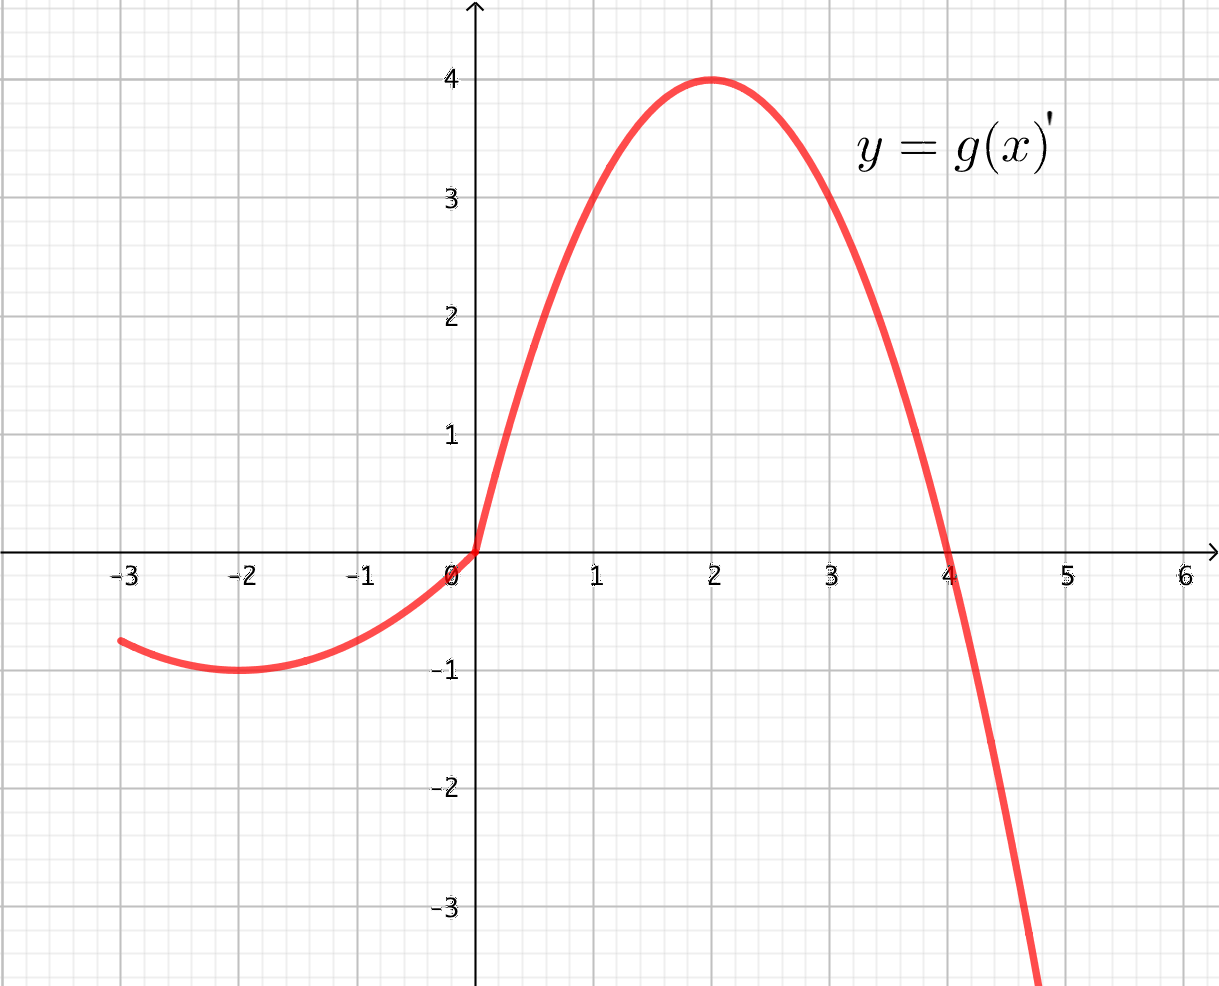
\includegraphics[width=0.8\textwidth]{gprima.png}
    \caption{Función $g'(x)$.\label{fig:gprima}}                           % EDIT - Create unique labels for figures
    \addtocounter{figure}{-1}
\end{figure}
En base a la figura~\Alph{numeroDeSecciones}\ref{fig:gprima} describiendo $g'(x)$, analice la función y responda las siguientes preguntas.

\begin{parts}
    % -----------------------------------------------------
    \part Determine dónde la derivada de $g(x)$ se anula.
    \mostrarpuntaje

    \begin{solution}
        Dado que se tiene el gráfico de la derivada ($g'(x)$), solo necesitamos buscar donde la ordenada es $0$, que en este caso es $x = 4$ y $x = 0$.
        % -----------------------------------------------------
        % To include a handwritten solution, scan or photograph
        % it and save it in the Images folder. Then use the
        % following code to include it in the exam paper,
        % simply change the name of the image file within the
        % \includegraphics LaTeX command.
        % -----------------------------------------------------
    \end{solution}

    % -----------------------------------------------------
    \part[5] Determine los intervalos de crecimiento y decrecimiento de $g(x)$.
    \mostrarpuntaje

    \begin{solution}
        Buscaremos los intervalos en donde nuestra derivada es positiva y negativa. Tenemos que tener mucho ojo en tomar valores en el eje $x$, puesto que justo ahí el valor de nuestra derivada es $0$. Dicho esto, el intervalo de crecimiento es $(0, 4)$ y decrece en $(-3, 0) \cup (4, 5)$.
    \end{solution}

    % -----------------------------------------------------
    \part[5] Determine la concavidad de $g(x)$ en el intervalo $(-3, 5)$.
    \mostrarpuntaje

    \begin{solution}
        Para calcular la concavidad, solo debemos analizar el signo de nuestra segunda derivada.

        En $(-3,-2) \cup (2,5)$ nuestra funcion es cóncava hacia abajo, puesto que $G''(x) < 0$.

        En el intervalo $(-2,2)$ nuestra $G''(x) > 0$, por lo que será cóncava hacia arriba.
    \end{solution}

    \part[5] Determine los máximos y mínimos locales de $g(x)$ en el dominio del gráfico.
    \mostrarpuntaje

    \begin{solution}
        Para determinar los puntos mínimos y maximos tenemos que analizar nuestra segunda derivada en los puntos críticos de la función, es decir, en donde nuestra primera derivada sea igual a $0$.\\

        Notamos que nuestra derivada es $0$ en $x=0$ y $x=4$, por lo que nos toca analizar el signo de nuestra segunda derivada en las cercanías de $x = 0$ y $x = 4$\\

        En $x=0$ nuestra G’’(x) es $>0$, por lo qué hay un mínimo local en $x=0$, $y = 0$.
    \end{solution}
\end{parts}
